\documentclass[12pt]{article}

% ========================== Packages ==========================
\usepackage[margin=1in]{geometry}
\usepackage{amsmath, amssymb, amsfonts, bm}
\usepackage{mathtools}
\usepackage{array, booktabs, multirow}
\usepackage{tikz}
\usetikzlibrary{arrows.meta,positioning,shapes.geometric,fit,calc}
\usepackage{enumitem}
\usepackage{xcolor}
\usepackage{hyperref}
\usepackage{fancyhdr}
\usepackage{titlesec}

% ========================== Page Setup ==========================
\setlength{\parskip}{0.65em}
\setlength{\parindent}{0pt}
\pagestyle{fancy}
\fancyhead[L]{\small ENGS 177: Decision Making Under Uncertainty}
\fancyhead[R]{\small Homework 1: Taka Khoo}
\fancyfoot[C]{\thepage}

\hypersetup{colorlinks=true,linkcolor=blue,urlcolor=blue,citecolor=blue}

\definecolor{chancefill}{RGB}{210,228,248}

\titleformat{\section}{\normalfont\Large\bfseries}{\thesection}{1em}{}
\titleformat{\subsection}{\normalfont\large\bfseries}{\thesubsection}{1em}{}

\newcommand{\R}{\mathbb{R}}
\newcommand{\EE}{\mathbb{E}}
\newcommand{\Prb}{\mathbb{P}}
\newcommand{\argmax}{\operatorname*{arg\,max}}
\newcommand{\argmin}{\operatorname*{arg\,min}}
\newcommand{\pa}{\operatorname{pa}}
\newcommand{\mat}[1]{\bm{#1}}

\tikzset{
  chance/.style={ellipse,draw,fill=chancefill,minimum width=12mm,minimum height=8mm,thick,inner sep=1pt},
}

\begin{document}

%=======================================================================
% TITLE
%=======================================================================
\begin{center}
  {\LARGE \textbf{ENGS 177: Decision Making Under Uncertainty}}\\[0.35em]
  {\Large \textbf{Homework 1}}\\[0.25em]
  \textbf{Name:} Taka Khoo \quad\textbullet\quad \textbf{Instructor:} Professor Wesley Marrero\\[0.25em]
  \textbf{Due:} April 17, 2026
\end{center}
\hrule
\vspace{0.25em}

\footnotesize\textit{Note: Claude (Anthropic) was used to sanity-check reasoning, verify arithmetic, and help polish the \LaTeX{} formatting.}
\normalsize
\vspace{0.5em}
\hrule
\vspace{0.75em}

%=======================================================================
\section*{Problem 1: White River Junction Train Station \hfill [20 pts]}
%=======================================================================

\textbf{Variables.} Four random variables, all with finite discrete state spaces:
\begin{itemize}[leftmargin=1.5em,itemsep=1pt]
  \item $T\in\{\text{day},\text{eve}\}$: time-of-day regime. Daytime is 6am to 6pm (12 hours), evening is 6pm to midnight (6 hours).
  \item $L\in\{65,23,18\}$: which line the arriving train belongs to.
  \item $S\in\{\text{short},\text{long}\}$: the train's physical setting.
  \item $D\in\{\text{Montreal},\text{NYC}\}$: the direction the train is headed (including depot runs, since the depot direction is given per line).
\end{itemize}

\subsection*{(a) Bayesian network [4 pts]}

``Short'' depends on both the line and the time (e.g.\ line~65 is short only in evenings). The direction depends on the line (every 10th train of each line goes to that line's depot). Time and line are modeled as independent (trains of all three lines run throughout the day). This gives the DAG
\[
  T\to S,\qquad L\to S,\qquad L\to D,
\]
which is a common-effect at $S$ plus a serial $L\to D$ structure.

\begin{center}
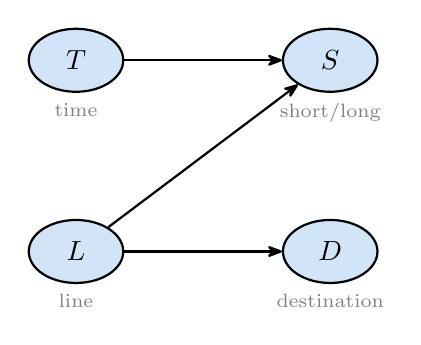
\begin{tikzpicture}[>={Stealth[round]},thick,node distance=1.6cm and 2.0cm]
  \node[chance] (T) {$T$};
  \node[chance,right=of T] (S) {$S$};
  \node[chance,below=of T] (L) {$L$};
  \node[chance,right=of L] (D) {$D$};
  \draw[->] (T) -- (S);
  \draw[->] (L) -- (S);
  \draw[->] (L) -- (D);
  \node[below=0pt of T,font=\scriptsize,gray] {time};
  \node[below=0pt of L,font=\scriptsize,gray] {line};
  \node[below=0pt of S,font=\scriptsize,gray] {short/long};
  \node[below=0pt of D,font=\scriptsize,gray] {destination};
\end{tikzpicture}
\end{center}
The joint factorizes as $\Prb(T,L,S,D)=\Prb(T)\,\Prb(L)\,\Prb(S\mid T,L)\,\Prb(D\mid L)$.

\subsection*{(b) Conditional probability tables [6 pts]}

\textbf{Prior on time $T$.} Assuming trains are distributed evenly in time,
\[
  \Prb(T=\text{day})=\tfrac{12}{18}=\tfrac{2}{3},\qquad \Prb(T=\text{eve})=\tfrac{6}{18}=\tfrac{1}{3}.
\]

\textbf{Prior on line $L$.} Given directly:
\[
  \Prb(L=65)=0.5,\quad \Prb(L=23)=0.3,\quad \Prb(L=18)=0.2.
\]

\textbf{CPT for $S\mid T,L$.} The problem states line~23 takes a long setting with probability $0.8$, so short with probability $0.2$; line~18 is short with probability $0.9$ during the daytime and always short during the evening; line~65 is short only in evenings with probability $0.1$.
\begin{center}
\begin{tabular}{ccc}
\toprule
$L$ & $T$ & $\Prb(S=\text{short}\mid T,L)$ \\
\midrule
$65$ & day & $0.0$ \\
$65$ & eve & $0.1$ \\
$23$ & day & $0.2$ \\
$23$ & eve & $0.2$ \\
$18$ & day & $0.9$ \\
$18$ & eve & $1.0$ \\
\bottomrule
\end{tabular}
\end{center}

\textbf{CPT for $D\mid L$.} Every 10th train goes to that line's depot (probability $0.1$). Line 23's depot is in the NYC direction, so a normal 23 goes to Montreal and a depot 23 goes to NYC. Lines 18, 65 have depots in the Montreal direction, so a normal 18/65 goes to NYC and a depot 18/65 goes to Montreal.
\begin{center}
\begin{tabular}{ccc}
\toprule
$L$ & $\Prb(D=\text{Montreal}\mid L)$ & $\Prb(D=\text{NYC}\mid L)$ \\
\midrule
$65$ & $0.1$ & $0.9$ \\
$23$ & $0.9$ & $0.1$ \\
$18$ & $0.1$ & $0.9$ \\
\bottomrule
\end{tabular}
\end{center}

\subsection*{(c) Evening, short train: probability Montreal-bound? [6 pts]}

We want $\Prb(D=\text{Montreal}\mid T=\text{eve},\,S=\text{short})$. Condition on $L$ and marginalize:
\[
  \Prb(D=\text{Mon}\mid T=\text{eve},S=\text{sh})
  = \sum_{\ell}\Prb(D=\text{Mon}\mid L=\ell)\,\Prb(L=\ell\mid T=\text{eve},S=\text{sh}).
\]

\textbf{Step 1: posterior over $L$ given (eve, short).} Using Bayes' rule and the independence $L\perp T$:
\[
  \Prb(L=\ell\mid T=\text{eve},S=\text{sh}) \;\propto\; \Prb(L=\ell)\,\Prb(S=\text{sh}\mid T=\text{eve},L=\ell).
\]
Compute each unnormalized score:
\begin{align*}
  L=65:\;&\Prb(L=65)\cdot\Prb(\text{sh}\mid \text{eve},65) = 0.5\cdot 0.1 = 0.05,\\
  L=23:\;&\Prb(L=23)\cdot\Prb(\text{sh}\mid \text{eve},23) = 0.3\cdot 0.2 = 0.06,\\
  L=18:\;&\Prb(L=18)\cdot\Prb(\text{sh}\mid \text{eve},18) = 0.2\cdot 1.0 = 0.20.
\end{align*}
Normalizing constant: $Z = 0.05+0.06+0.20 = 0.31$. Posterior:
\[
  \Prb(L=65\mid \cdot)=\tfrac{0.05}{0.31}\approx 0.1613,\quad
  \Prb(L=23\mid \cdot)=\tfrac{0.06}{0.31}\approx 0.1935,\quad
  \Prb(L=18\mid \cdot)=\tfrac{0.20}{0.31}\approx 0.6452.
\]

\textbf{Step 2: weight by $\Prb(\text{Montreal}\mid L)$.}
\[
  \Prb(D=\text{Mon}\mid \text{eve},\text{sh})
  = \frac{0.05\cdot 0.1 + 0.06\cdot 0.9 + 0.20\cdot 0.1}{0.31}
  = \frac{0.005 + 0.054 + 0.020}{0.31}
  = \frac{0.079}{0.31}.
\]

\textbf{Final answer.}
\[
  \Prb(D=\text{Montreal}\mid T=\text{evening},S=\text{short}) \;=\; \tfrac{0.079}{0.31}\;\approx\;0.2548\ (\approx 25.5\%).
\]
A short evening train is most likely line 18 (always short in the evening), and line 18's default direction is NYC, so a Montreal probability below one third is reasonable.

\subsection*{(d) Train 65 arrived. $\Prb(S\mid L=65)$? [4 pts]}

Marginalize $T$ from the CPT using the law of total probability:
\begin{align*}
  \Prb(S=\text{sh}\mid L=65)
  &= \Prb(S=\text{sh}\mid \text{day},65)\Prb(\text{day}) + \Prb(S=\text{sh}\mid \text{eve},65)\Prb(\text{eve})\\
  &= 0\cdot\tfrac{2}{3} + 0.1\cdot\tfrac{1}{3} \;=\; \tfrac{1}{30}\approx 0.0333.
\end{align*}
Therefore
\[
  \Prb(S=\text{short}\mid L=65)=\tfrac{1}{30}\approx 0.033,\qquad
  \Prb(S=\text{long}\mid L=65)=\tfrac{29}{30}\approx 0.967.
\]
Line~65 is almost certainly long if observed: it is only ever short (with low probability) during evenings, which occupy a minority of the operating day.

%=======================================================================
\section*{Problem 2: Smart-Home Alarm Bayesian Network \hfill [20 pts]}
%=======================================================================

\subsection*{(a) Draw + conditional-independence via d-separation [8 pts]}

\begin{center}
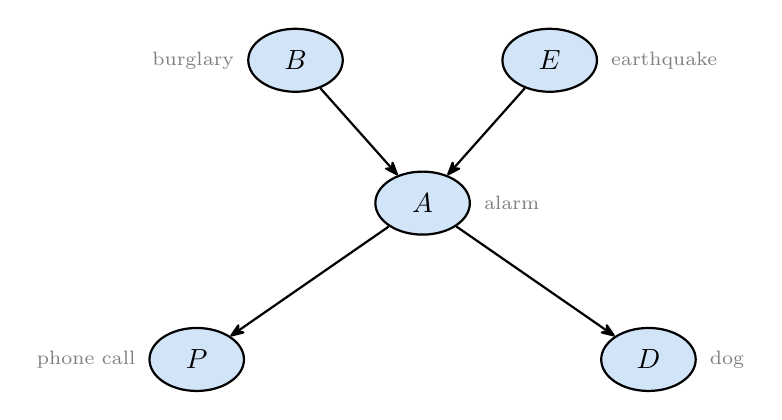
\begin{tikzpicture}[>={Stealth[round]},thick,node distance=1.4cm and 2.0cm]
  \node[chance] (B) {$B$};
  \node[chance,right=of B] (E) {$E$};
  \node[chance,below=of $(B)!0.5!(E)$] (A) {$A$};
  \node[chance,below left=of A] (P) {$P$};
  \node[chance,below right=of A] (D) {$D$};
  \draw[->] (B) -- (A);
  \draw[->] (E) -- (A);
  \draw[->] (A) -- (P);
  \draw[->] (A) -- (D);
  \node[left=1pt of B,font=\scriptsize,gray] {burglary};
  \node[right=1pt of E,font=\scriptsize,gray] {earthquake};
  \node[right=1pt of A,font=\scriptsize,gray] {alarm};
  \node[left=1pt of P,font=\scriptsize,gray] {phone call};
  \node[right=1pt of D,font=\scriptsize,gray] {dog};
\end{tikzpicture}
\end{center}

Factorization: $\Prb(B,E,A,P,D)=\Prb(B)\Prb(E)\Prb(A\mid B,E)\Prb(P\mid A)\Prb(D\mid A)$.

\textbf{Conditional-independence properties via d-separation.} Applying the three connection rules:
\begin{itemize}[leftmargin=1.5em,itemsep=3pt]
  \item \textbf{$B\perp E$ (unconditional).} The only path between $B$ and $E$ is $B\to A\leftarrow E$, a common-effect (v-structure, collider) at $A$. Colliders block paths unless the collider (or a descendant) is observed. With no evidence, $A$ is unobserved, so the path is blocked. Hence $B\perp E$.
  \item \textbf{$B\not\perp E\mid A$ (explaining away).} Conditioning on the collider $A$ opens the path $B\to A\leftarrow E$. Intuitively: if the alarm sounds and an earthquake is known to have happened, that explains away the alarm and decreases belief in burglary.
  \item \textbf{$P\perp D\mid A$.} The only path between $P$ and $D$ is $P\leftarrow A\to D$, a common-cause (divergent) connection at $A$. Conditioning on $A$ blocks it, so $P\perp D\mid A$. Without conditioning on $A$, $P$ and $D$ are dependent (both are downstream of $A$).
  \item \textbf{$B\perp P\mid A$ and $B\perp D\mid A$.} The paths $B\to A\to P$ and $B\to A\to D$ are serial connections through $A$; conditioning on $A$ blocks them. Once the alarm state is known, burglary tells us nothing further about phone calls or barking.
  \item The same argument gives $E\perp P\mid A$ and $E\perp D\mid A$.
\end{itemize}

\subsection*{(b) Compute $\Prb(B=1\mid P=1,D=1)$ [12 pts]}

By Bayes' rule,
\[
  \Prb(B=1\mid P=1,D=1) \;=\; \frac{\Prb(B=1,P=1,D=1)}{\Prb(P=1,D=1)},
\]
and both terms are obtained by marginalizing $E$ and $A$ out of the joint. Two reductions keep the arithmetic clean.

\paragraph{Reduction 1: marginalize $E$ into $\Prb(A\mid B)$.}
\begin{align*}
  \Prb(A=1\mid B=1) &= \Prb(A=1\mid B=1,E=1)\Prb(E=1)+\Prb(A=1\mid B=1,E=0)\Prb(E=0)\\
  &= 0.95(0.02)+0.94(0.98) = 0.019+0.9212 = 0.9402,\\
  \Prb(A=1\mid B=0) &= 0.29(0.02)+0.001(0.98) = 0.0058+0.00098 = 0.00678.
\end{align*}
So $\Prb(A=0\mid B=1)=0.0598$ and $\Prb(A=0\mid B=0)=0.99322$.

\paragraph{Reduction 2: collapse $P,D$ into a single factor.} Because $P\perp D\mid A$,
\[
  \Prb(P=1,D=1\mid A) = \Prb(P=1\mid A)\,\Prb(D=1\mid A).
\]
Hence
\[
  \Prb(P=1,D=1\mid A=1)=0.9\cdot 0.7=0.63,\qquad
  \Prb(P=1,D=1\mid A=0)=0.05\cdot 0.2=0.01.
\]

\paragraph{Numerator.}
\begin{align*}
  \Prb(B=1,P=1,D=1)
  &= \Prb(B=1)\sum_{a}\Prb(A=a\mid B=1)\,\Prb(P=1,D=1\mid A=a)\\
  &= 0.01\bigl[\,0.9402\cdot 0.63 + 0.0598\cdot 0.01\,\bigr]\\
  &= 0.01\bigl[\,0.592326 + 0.000598\,\bigr]\\
  &= 0.01\cdot 0.592924 = 0.00592924.
\end{align*}

\paragraph{Denominator.} Also need the $B=0$ term:
\begin{align*}
  \Prb(B=0,P=1,D=1)
  &= 0.99\bigl[\,0.00678\cdot 0.63 + 0.99322\cdot 0.01\,\bigr]\\
  &= 0.99\bigl[\,0.0042714 + 0.0099322\,\bigr]\\
  &= 0.99\cdot 0.0142036 = 0.01406156.
\end{align*}
Summing,
\[
  \Prb(P=1,D=1)=0.00592924+0.01406156 = 0.0199908.
\]

\paragraph{Final ratio.}
\[
  \Prb(B=1\mid P=1,D=1)=\frac{0.00592924}{0.0199908}\approx 0.29660.
\]

\textbf{Final answer.} $\Prb(B=1\mid P=1,D=1)\approx 0.2966\ (\approx 29.7\%)$. The prior is $\Prb(B=1)=0.01$; observing both a phone call and a barking dog pushes the posterior up by a factor of about $30$, as two independent noisy indicators of an alarm strongly corroborate each other.

%=======================================================================
\section*{Problem 3: Rabbit Genetics Markov Chain \hfill [20 pts]}
%=======================================================================

\subsection*{(a) Transition probabilities [6 pts]}

Let $X_n\in\{GG,Gg,gg\}$ be the genotype of the $n$-th-generation rabbit. Each generation, $X_n$ is mated with a fresh hybrid $Gg$. The offspring gets one allele from each parent, independently and uniformly from that parent's pair.

\textbf{From $X_n=GG$ (alleles $G,G$) $\times$ $Gg$.} The $GG$ parent gives $G$ deterministically; the $Gg$ parent gives $G$ w.p.\ $1/2$ and $g$ w.p.\ $1/2$. Offspring: $GG$ w.p.\ $1/2$, $Gg$ w.p.\ $1/2$.

\textbf{From $X_n=Gg\times Gg$.} Each parent independently gives $G$ or $g$ w.p.\ $1/2$. Offspring:
\[
  \Prb(GG)=\tfrac12\cdot\tfrac12=\tfrac14,\quad \Prb(Gg)=2\cdot\tfrac12\cdot\tfrac12=\tfrac12,\quad \Prb(gg)=\tfrac14.
\]

\textbf{From $X_n=gg\times Gg$.} The $gg$ parent gives $g$ always; the $Gg$ parent gives $G$ w.p.\ $1/2$, $g$ w.p.\ $1/2$. Offspring: $Gg$ w.p.\ $1/2$, $gg$ w.p.\ $1/2$.

Assembling in row order $(GG,Gg,gg)$, the transition matrix is
\[
  \mat{P}=\begin{pmatrix}
    1/2 & 1/2 & 0 \\
    1/4 & 1/2 & 1/4 \\
    0   & 1/2 & 1/2
  \end{pmatrix}.
\]
Each row sums to $1$. Graphically:
\begin{center}
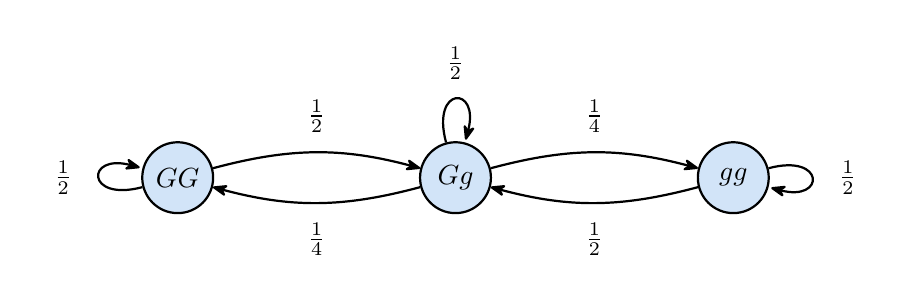
\begin{tikzpicture}[->,>={Stealth[round]},thick, node distance=2.6cm,
  every node/.style={circle,draw,fill=chancefill,minimum size=9mm,inner sep=0pt}]
  \node (GG) {$GG$};
  \node[right=of GG] (Gg) {$Gg$};
  \node[right=of Gg] (gg) {$gg$};
  \draw (GG) edge[loop left] node[draw=none,fill=none,left]{$\tfrac12$} (GG);
  \draw (gg) edge[loop right] node[draw=none,fill=none,right]{$\tfrac12$} (gg);
  \draw (Gg) edge[loop above] node[draw=none,fill=none,above]{$\tfrac12$} (Gg);
  \draw (GG) edge[bend left=15] node[draw=none,fill=none,above]{$\tfrac12$} (Gg);
  \draw (Gg) edge[bend left=15] node[draw=none,fill=none,below]{$\tfrac14$} (GG);
  \draw (Gg) edge[bend left=15] node[draw=none,fill=none,above]{$\tfrac14$} (gg);
  \draw (gg) edge[bend left=15] node[draw=none,fill=none,below]{$\tfrac12$} (Gg);
\end{tikzpicture}
\end{center}

\subsection*{(b) $\mu_1,\mu_2,\mu_3$ and $\mu_n$ in general [14 pts]}

Start with a hybrid: $\mu_0=(0,1,0)$ (as a row vector in the order $GG,Gg,gg$). Using the row-stochastic convention $\mu_{n+1}=\mu_n\mat{P}$:

\paragraph{Compute $\mu_1$.}
\[
  \mu_1 = \mu_0 \mat{P}
  = (0,1,0)\!\begin{pmatrix}1/2 & 1/2 & 0\\ 1/4 & 1/2 & 1/4\\ 0 & 1/2 & 1/2\end{pmatrix}
  = \Bigl(\tfrac14,\;\tfrac12,\;\tfrac14\Bigr).
\]
(Simply the second row of $\mat P$.)

\paragraph{Compute $\mu_2$.} Coordinate by coordinate:
\begin{align*}
  \mu_2(GG) &= \tfrac14\cdot\tfrac12 + \tfrac12\cdot\tfrac14 + \tfrac14\cdot 0 = \tfrac18+\tfrac18 = \tfrac14,\\
  \mu_2(Gg) &= \tfrac14\cdot\tfrac12 + \tfrac12\cdot\tfrac12 + \tfrac14\cdot\tfrac12 = \tfrac18+\tfrac14+\tfrac18 = \tfrac12,\\
  \mu_2(gg) &= \tfrac14\cdot 0 + \tfrac12\cdot\tfrac14 + \tfrac14\cdot\tfrac12 = \tfrac18+\tfrac18 = \tfrac14.
\end{align*}
So $\mu_2=(1/4,1/2,1/4)$, identical to $\mu_1$.

\paragraph{General $n$.} Since $\mu_1\mat{P}=\mu_1$, the distribution $\mu_1=(1/4,1/2,1/4)$ is a stationary distribution of $\mat P$. Therefore
\[
  \mu_n = \mu_1 = (1/4,\;1/2,\;1/4)\qquad\text{for every }n\ge 1.
\]
In particular $\mu_3=(1/4,1/2,1/4)$. A direct check:
\[
  \mu_3(GG)=\tfrac14\cdot\tfrac12+\tfrac12\cdot\tfrac14+\tfrac14\cdot 0 = \tfrac14,\quad\text{etc.}\;\checkmark
\]

\textbf{Final answer.}
\[
  \mu_1=\mu_2=\mu_3=\cdots=\mu_n=\Bigl(\tfrac14,\tfrac12,\tfrac14\Bigr)\qquad\text{for all }n\ge 1.
\]
After one mating with a hybrid, the offspring of a hybrid sits at a Hardy--Weinberg-like equilibrium: allele frequencies are $\Prb(G)=\Prb(g)=\tfrac12$ and the three genotypes are in the $1{:}2{:}1$ ratio predicted by random mating. Because each generation is mated against a hybrid, keeping allele frequencies fixed, subsequent generations stay in this equilibrium forever.

%=======================================================================
\section*{Problem 4: Random Walk on a Cube \hfill [20 pts]}
%=======================================================================

Label the eight corners $\{0,1\}^3$ so that corner $i=(0,0,0)$ and opposite corner $o=(1,1,1)$. From each corner the bug moves to one of the $3$ adjacent corners uniformly (adjacency = differ in exactly one bit).

\subsection*{(a) Long-run fraction of time at $i$ [10 pts]}

\textbf{Symmetry argument.} The cube's automorphism group acts transitively on its corners: for any two corners $u,v$, there is a graph automorphism mapping $u\mapsto v$ (flip coordinates / permute axes). Since the transition matrix is determined by the cube's adjacency structure alone, any automorphism $\sigma$ satisfies $\mat P_{\sigma(u)\sigma(v)}=\mat P_{uv}$. Hence the stationary distribution $\pi$ (unique for an irreducible finite chain) is invariant under $\sigma$. Since any corner can be mapped to any other, $\pi$ must be uniform:
\[
  \pi_v = \tfrac{1}{8}\qquad\forall v\in\{0,1\}^3.
\]

The same conclusion follows from detailed balance. The cube graph is $3$-regular, so for any edge $(u,v)$, $\tfrac{1}{8}\cdot\tfrac{1}{3}=\tfrac{1}{8}\cdot\tfrac{1}{3}$; the uniform distribution satisfies $\pi_u p_{uv}=\pi_v p_{vu}$, confirming that $\pi=(\tfrac18,\dots,\tfrac18)$ is stationary. By uniqueness, this is the answer.

\textbf{Final answer.} The long-run proportion of time the bug spends at corner $i$ is $\pi_i=\tfrac{1}{8}$.

Note that the cube graph is bipartite (partition corners by parity of the bit-sum), so the chain has period $2$. The limiting probabilities $\lim_n p_{ij}^{(n)}$ therefore do not exist. Long-run proportions (time averages) are, however, well-defined for irreducible finite chains regardless of period, and they equal the unique stationary distribution.

\subsection*{(b) Expected number of steps until first visit to $o$ [10 pts]}

\textbf{State-reduction by distance.} Group corners by Hamming distance from $i$:
\begin{itemize}[leftmargin=1.5em,itemsep=1pt]
  \item Class $0$: $\{i\}$ (1 corner, bit-sum $0$).
  \item Class $1$: $3$ neighbors of $i$ (bit-sum $1$).
  \item Class $2$: $3$ antipodal neighbors (bit-sum $2$).
  \item Class $3$: $\{o\}$ (1 corner, bit-sum $3$).
\end{itemize}
From class $0$, all $3$ moves go to class $1$. From a class-$1$ corner, $1$ of the $3$ neighbors is $i$ (flip the one $1$ back to $0$) and the other $2$ are class-$2$ corners (flip either of the $0$-coordinates). From a class-$2$ corner, symmetrically, $1$ neighbor is $o$ and $2$ are class-$1$. From $o$, the target has been hit. The distance process is itself a Markov chain on $\{0,1,2,3\}$ with transitions
\[
  0\to 1\ (\text{prob }1),\quad 1\to\{0,2\}\ (\text{probs }\tfrac13,\tfrac23),\quad 2\to\{1,3\}\ (\text{probs }\tfrac23,\tfrac13),\quad 3\to 3.
\]

\textbf{Hitting-time equations.} Let $k_d$ be the expected number of steps to reach $o$ (class $3$) starting from a corner in class $d$. Boundary: $k_3=0$. Interior:
\begin{align*}
  k_0 &= 1 + k_1,\\
  k_1 &= 1 + \tfrac13 k_0 + \tfrac23 k_2,\\
  k_2 &= 1 + \tfrac23 k_1 + \tfrac13\cdot 0 = 1+\tfrac23 k_1.
\end{align*}

\textbf{Solve.} Substitute $k_0=1+k_1$ into the equation for $k_1$:
\[
  k_1 = 1 + \tfrac13(1+k_1) + \tfrac23 k_2 \Longrightarrow k_1 - \tfrac13 k_1 = \tfrac43 + \tfrac23 k_2
  \Longrightarrow \tfrac23 k_1 = \tfrac43+\tfrac23 k_2 \Longrightarrow k_1 = 2 + k_2.
\]
Substitute into $k_2=1+\tfrac23 k_1$:
\[
  k_2 = 1+\tfrac23(2+k_2) = 1+\tfrac43+\tfrac23 k_2 \Longrightarrow \tfrac13 k_2 = \tfrac73 \Longrightarrow k_2 = 7.
\]
Then $k_1=2+7=9$ and $k_0=1+k_1=10$.

\textbf{Final answer.} Starting from $i$, the expected number of steps until the bug first visits $o$ is $\EE_i[H_o] = k_0 = 10$ steps. As a consistency check, the mean return time to any corner under uniform $\pi$ is $1/\pi_v=8$ (Kac's lemma); reaching the specific farthest corner is slightly longer than a generic return.

%=======================================================================
\section*{Problem 5: Term Project Preliminary Description \hfill [20 pts]}
%=======================================================================

\textbf{Working title:} \emph{Inventory Management under Uncertain Demand and Lead Times.}

We consider a single-product inventory system in which the operator must decide, at each review period $t$, whether and how much to restock. Let $s_t$ denote the inventory level at the start of period $t$, $D_t$ the random customer demand during period $t$, and $L_t$ the random supplier lead time for any order placed in that period.

\subsection*{(a) Decisions and alternatives [5 pts]}

At each period $t$ the operator chooses two interacting quantities that together define the ordering policy:
\begin{itemize}[leftmargin=1.5em,itemsep=2pt]
  \item The \textbf{reorder point} $R$: the inventory level at which a new order is triggered. When $s_t \le R$, an order is placed; when $s_t > R$, no order is placed.
  \item The \textbf{reorder quantity} $Q$: how many units are ordered when the reorder point is hit.
\end{itemize}
This is the classical $(R, Q)$ policy structure from operations research. The alternatives form a two-dimensional continuum, since any combination of reorder point $R \in \{0, 1, \dots, M\}$ and reorder quantity $Q \in \{1, \dots, M - R\}$ is feasible, where $M$ is the maximum storage capacity. Each $(R, Q)$ pair trades off ordering frequency against holding cost and the risk of stockout differently; the optimal pair depends on the specific cost structure (ordering, holding, shortage) and the demand and lead-time distributions.

\subsection*{(b) Sources of uncertainty [5 pts]}

The problem has three interacting sources of uncertainty:
\begin{enumerate}[leftmargin=1.5em,itemsep=2pt]
  \item \textbf{Customer demand} $D_t$: the number of units requested per period. Typically modeled as an i.i.d.\ random variable drawn from a distribution $f_D$ estimated from historical sales data.
  \item \textbf{Supplier lead time} $L_t$: the number of periods between placing an order and receiving it. Uncertain lead times mean that orders placed at time $t$ may arrive at $t+1$, $t+2$, or later, complicating the state dynamics.
  \item \textbf{Demand surges}: unexpected spikes in $D_t$ that can cause stockouts. These are fat-tail events not well captured by the bulk of $f_D$ and often require separate modeling (for example as a rare mixture component).
\end{enumerate}

\subsection*{(c) How to model the uncertainty [10 pts]}

\textbf{Proposed approach: a Markov chain on inventory levels.} Treat the inventory level $s_t$ as the state of a discrete-time stochastic process, exactly as in the inventory-control MDP introduced in Lecture~5. With a fixed $(R, Q)$ policy, the inventory evolves as
\[
  s_{t+1} \;=\; \max\!\left(s_t + a_t - D_t,\; 0\right),
\]
where $a_t = Q$ if $s_t \le R$ and $a_t = 0$ otherwise, and $D_t \sim f_D$ independently across periods. Because $s_{t+1}$ depends on the past only through $s_t$ (given the policy), the process $\{s_t\}$ is a Markov chain on the finite state space $\{0, 1, \dots, M\}$. Its transition matrix $\mat{P}^{(R,Q)}$ is determined entirely by $f_D$ and the policy, and its stationary distribution $\pi^{(R,Q)}$ gives the long-run proportion of time spent at each inventory level, which we can use to compute the long-run average cost per period.

If we want to capture random lead times as well, we enlarge the state to include outstanding orders, for example $s_t = (\text{on-hand},\, \text{pipeline})$ where ``pipeline'' tracks orders placed but not yet received. This is exactly the process-transformation trick from Lecture~3: when memory extends beyond a single scalar, enlarge the state until the Markov property holds.

The demand distribution $f_D$ would be estimated from historical sales, either empirically (as the observed frequency of each demand value) or by fitting a parametric family such as Poisson or negative binomial.

\textbf{Why not a Bayesian network?} The relationships between inventory level, reorder point, and reorder quantity are deterministic once the policy is fixed, and the main modeling difficulty is the \emph{operational, sequential} nature of the decision rather than a static conditional-independence structure. A Bayesian network would model uncertainty at one period but would not capture how inventory evolves from period to period or how the choice of $(R, Q)$ propagates through time.

\textbf{Summary.} Model the inventory level as the state of a discrete-time Markov chain on $\{0, 1, \dots, M\}$, with transition probabilities induced by the chosen $(R, Q)$ policy and the estimated demand distribution. If lead times are uncertain, enlarge the state to include the order pipeline. Evaluating the long-run average cost under candidate policies (via the stationary distribution) and selecting the $(R, Q)$ pair that minimizes this cost is exactly the formulation we will use in Part~III when we introduce Markov decision processes for this kind of problem.

\end{document}
